% Name: Borromean rings
% Description: Three rings linked so that each lies over the next and under the one before it: no two are linked, yet the three cannot be pulled apart.
% Tags: Borromean rings, link, knot theory, Brunnian link

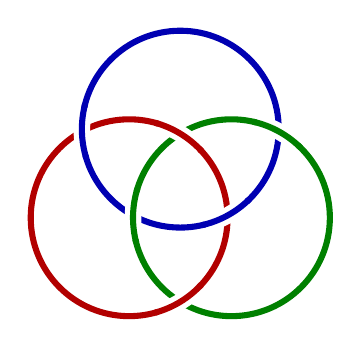
\begin{tikzpicture}[line width=2.2pt]
  % Centers 0.75 from the origin at 90°, 210°, and 330°, radius 1.25; the crossings were solved for their angles on each ring
  \foreach \c/\a in {blue!70!black/90, red!70!black/210, green!50!black/330} \draw[\c] (\a:0.75) circle (1.25);
  % Each ring is on top at both of its crossings with the next: blue over red, red over green, green over blue
  \foreach \c/\a/\t in {blue!70!black/90/-61.3, blue!70!black/90/-178.7, red!70!black/210/58.7, red!70!black/210/-58.7, green!50!black/330/178.7, green!50!black/330/61.3} {
    \draw[white, line width=6pt] (\a:0.75) ++(\t-14:1.25) arc[start angle=\t-14, end angle=\t+14, radius=1.25];
    \draw[\c] (\a:0.75) ++(\t-16:1.25) arc[start angle=\t-16, end angle=\t+16, radius=1.25];
  }
\end{tikzpicture}
